\documentclass[tikz,border=2pt,11pt]{standalone}
\usetikzlibrary{arrows.meta}
\usetikzlibrary{shapes.geometric}
\usetikzlibrary{patterns}
\usetikzlibrary{calc}
\usepackage{amsmath}
\usepackage{amssymb}
\usepackage{graphicx}
\usepackage{xcolor}
\usepackage{tikz}
\newcommand{\PP}{\mathbb P}
\newcommand{\EE}{\mathbb E}
\newcommand{\pc}{p_c}
\newcommand{\R}{\mathbb R}
\newcommand{\Z}{\mathbb Z}
\newcommand{\N}{\mathbb N}
\DeclareMathOperator{\Var}{Var}
\DeclareMathOperator{\Cov}{Cov}
\DeclareMathOperator{\Ent}{Ent}
\DeclareMathOperator{\Aut}{Aut}
\DeclareMathOperator{\osc}{osc}
\DeclareMathOperator{\dist}{dist}
\begin{document}
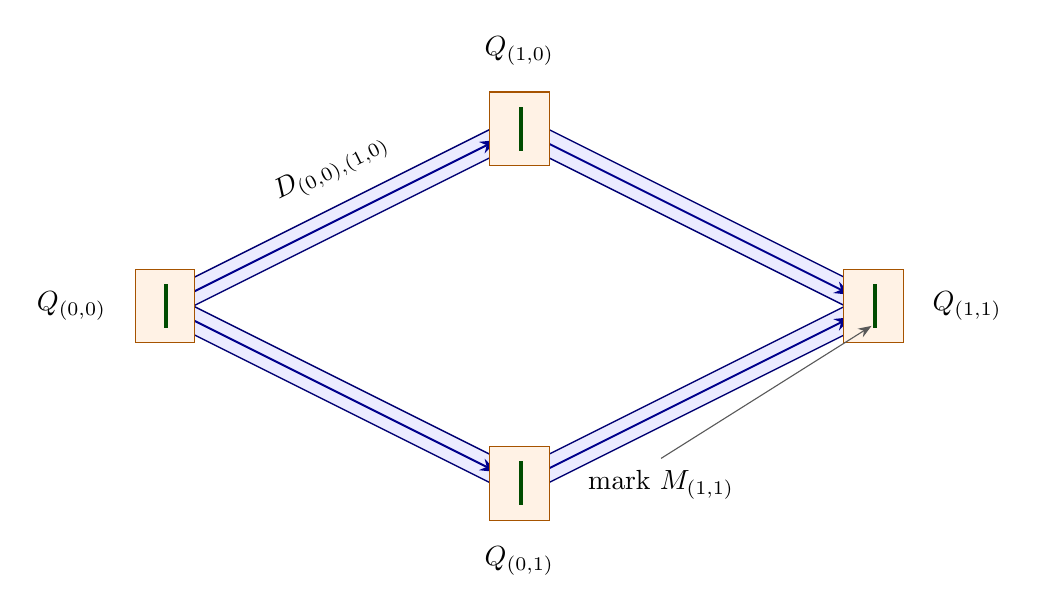
\begin{tikzpicture}[x=.9cm,y=.9cm,>=Stealth]
 \foreach \ax/\ay/\bx/\by in {0/0/5/2.5,0/0/5/-2.5,5/2.5/10/0,5/-2.5/10/0}{
  \filldraw[fill=blue!8,draw=blue!45!black,line width=.5pt]
    (\ax,{\ay+.2})--(\bx,{\by+.2})--(\bx,{\by-.2})--(\ax,{\ay-.2})--cycle;
  \draw[->,blue!55!black,line width=.7pt,shorten <=9pt,shorten >=9pt]
    (\ax,\ay)--(\bx,\by);
 }
 \foreach \ax/\ay in {0/0,5/2.5,5/-2.5,10/0}{
  \filldraw[fill=orange!10,draw=orange!65!black]
    ({\ax-.42},{\ay-.52}) rectangle ({\ax+.42},{\ay+.52});
  \filldraw[fill=green!30!black,draw=green!30!black]
    (\ax,{\ay-.3}) rectangle ({\ax+.04},{\ay+.3});
 }
 \node[left=7pt] at (-.42,0) {$Q_{(0,0)}$};
 \node[above=6pt] at (5,3.02) {$Q_{(1,0)}$};
 \node[below=6pt] at (5,-3.02) {$Q_{(0,1)}$};
 \node[right=7pt] at (10.42,0) {$Q_{(1,1)}$};
 \node[above=4pt,rotate=26.565] at (2.5,1.48) {$D_{(0,0),(1,0)}$};
 \draw[->,black!65] (7,-2.15)--(9.97,-.28);
 \node[below,align=center] at (7,-2.18) {mark $M_{(1,1)}$};
\end{tikzpicture}
\end{document}
